\documentclass[12pt]{report}
\usepackage[utf8]{inputenc}
\usepackage{graphicx}
\graphicspath{{images/}}

\usepackage{listings}
\usepackage[british]{babel}
\usepackage{csquotes}
\usepackage[backend=biber,style=apa,sorting=nyt,natbib=true]{biblatex}
\DeclareLanguageMapping{british}{british-apa}
\addbibresource{references.bib}

\usepackage{geometry}
\usepackage{pdflscape}

% df2latex % objectivePerformanceDescriptivesTrim %  % objective measures of performance % 6objectiveTournamentDescriptives.tex


\title{
{Discussion Section}\\
{\large University of Oxford}
}
\author{Jacob Taylor}

%---------------------------------------------

\begin{document}

\maketitle{}

Almost all movement in this particular sporting context is generated in coordination with teammates or against opponents. The coordination of movement with others—“joint-action”—requires individuals to generate predictions that rely on the commitment of teammates (and opponents) to more or less the same action.  Successful coordination of group-specific joint-action generates mutual commitment between teammates over time, as individuals’ predictions about movement depend for their accuracy on the participation of others.\\

% df2latex % competenceDescriptivesTrim % 1competenceDescriptives.tex
\begin{table}[htpb]\caption{df2latex}
\begin{center}
\begin{scriptsize}
\begin{tabular} {l r r r r r r r }
 \multicolumn{ 7 }{l}{  } \cr
 \hline Variable  &   n  &  mean  &  sd  &  min  &  max  &  skew  &  krtss \cr
  \hline
yearsTeam   &  120  &   3.17  &   2.12  &    0  &   7  &   0.29  &  -1.25 \cr
 trainingAge   &  120  &   4.40  &   2.35  &    0  &  13  &   0.47  &   0.66 \cr
 startingAvg   &  172  &   0.61  &   0.36  &    0  &   1  &  -0.43  &  -1.32 \cr
 age   &  121  &  21.67  &   3.26  &   16  &  32  &   0.52  &  -0.27 \cr
 \\
 abilityTeammatesBaseline   &  120  &  19.45  &  20.14  &  -40  &  50  &  -0.31  &  -0.56 \cr
 abilityChineseProsBaseline   &  120  &  15.78  &  19.59  &  -35  &  50  &  -0.18  &  -0.65 \cr
 abilityInternationalProsBaseline   &  120  &  18.46  &  26.19  &  -44  &  50  &  -0.48  &  -0.77 \cr
 teamAbilityChineseProvincesBaseline   &  120  &  22.48  &  22.90  &  -40  &  50  &  -0.64  &  -0.58 \cr
 \hline
\end{tabular}
\end{scriptsize}
\end{center}
\label{post-Tournament measures of technical competence (objective and subjective)}
\end{table}

\begin{table}[htpb]\caption{df2latex}
\begin{center}
\begin{scriptsize}
\begin{tabular} {l r r r r r r r }
 \multicolumn{ 7 }{l}{  } \cr
 \hline Variable  &   n  &  mean  &  sd  &  min  &  max  &  skew  &  krtss \cr
  \hline
indPerformance7   &  118  &  56.36  &  23.47  &  0  &  100  &  -0.35  &  -0.08 \cr
 passingTech7   &  118  &  58.41  &  24.25  &  0  &  100  &  -0.79  &   0.05 \cr
 supportAttack7   &  118  &  62.62  &  22.70  &  0  &  100  &  -0.98  &   0.64 \cr
 indDefense7   &  118  &  57.64  &  23.57  &  0  &  100  &  -0.55  &  -0.11 \cr
 effectContact7   &  118  &  62.15  &  24.81  &  0  &  100  &  -0.97  &   0.40 \cr
 decisionAttack7   &  118  &  61.22  &  21.43  &  0  &  100  &  -0.72  &   0.37 \cr
 teamPerformance7   &  118  &  64.36  &  23.61  &  0  &  100  &  -0.52  &  -0.30 \cr
 teamDefense7   &  118  &  62.42  &  22.50  &  0  &  100  &  -0.52  &  -0.52 \cr
 teamAttack7   &  118  &  65.33  &  20.26  &  0  &  100  &  -0.53  &  -0.23 \cr
 teamSupportPlay7   &  118  &  65.75  &  19.72  &  0  &  100  &  -0.76  &   0.57 \cr
 teamCommunication7   &  118  &  65.25  &  21.26  &  0  &  100  &  -0.65  &   0.27 \cr
 \hline
\end{tabular}
\end{scriptsize}
\end{center}
\label{post-Tournament measures of performance (individual and team)}
\end{table}

% df2latex % clickPostDescriptivesTrim %  % post-Tournament measures of team click % 3clickPostDescriptives.tex
\begin{table}[htpb]\caption{df2latex}
\begin{center}
\begin{scriptsize}
\begin{tabular} {l r r r r r r r }
 \multicolumn{ 7 }{l}{  } \cr
 \hline Variable  &   n  &  mean  &  sd  &  min  &  max  &  skew  &  krtss \cr
  \hline
unspokenUnderstanding7   &  118  &  72.72  &  19.95  &  0  &  100  &  -1.38  &  2.13 \cr
 generalAtmosphere7   &  118  &  78.45  &  21.34  &  0  &  100  &  -1.51  &  2.82 \cr
 clickPictorial7   &  118  &   3.93  &   1.04  &  1  &    5  &  -0.78  &  0.00 \cr
 reliabilityOfOthers7   &  118  &  68.00  &  23.09  &  0  &  100  &  -1.33  &  1.75 \cr
 reliabilityForOthers7   &  118  &  63.45  &  25.80  &  0  &  100  &  -1.06  &  0.51 \cr
 abilityExtended7   &  118  &  72.25  &  19.27  &  0  &  100  &  -1.13  &  2.03 \cr
 \hline
\end{tabular}
\end{scriptsize}
\end{center}
\label{post-Tournament measures of team click}
\end{table}


%df2latex % bondingPostDescriptivesTrim %  % post-Tournament measures of social bonding % 4bondingPostDescriptives.tex
\begin{table}[htpb]\caption{df2latex}
\begin{center}
\begin{scriptsize}
\begin{tabular} {l r r r r r r r }
\multicolumn{ 7 }{l}{  } \cr
\hline Variable  &   n  &  mean  &  sd  &  min  &  max  &  skew  &  krtss \cr
 \hline
emotionalSupport7   &  118  &  79.67  &  18.84  &   0.00  &  100  &  -1.74  &  4.37 \cr
sharedGoal7   &  118  &  86.00  &  15.56  &  29.00  &  100  &  -1.38  &  2.24 \cr
groupId7   &  118  &   4.29  &   0.67  &   1.50  &    5  &  -1.18  &  1.66 \cr
fusionVerbal7   &  118  &   4.00  &   0.71  &   1.43  &    5  &  -0.86  &  0.99 \cr
fusionPictorialTeam7   &  118  &   4.33  &   1.19  &   0.00  &    5  &  -2.45  &  6.07 \cr
\hline
\end{tabular}
\end{scriptsize}
\end{center}
\label{post-Tournament measures of social bonding}
\end{table}




\begin{table}[htpb]\caption{df2latex}
\begin{center}
\begin{scriptsize}
\begin{tabular} {l r r r r r r r }
 \multicolumn{ 7 }{l}{  } \cr
 \hline Variable  &   n  &  mean  &  sd  &  min  &  max  &  skew  &  krtss \cr
  \hline
fatigue7   &  118  &  69.27  &  21.24  &   0  &  100  &  -1.13  &  1.40 \cr
 prpe7   &  118  &  14.97  &   2.66  &   6  &   20  &  -0.80  &  0.49 \cr
 mental7   &  118  &   6.08  &   2.47  &  -4  &   10  &  -1.13  &  1.82 \cr
 injury7   &  118  &  76.14  &  26.91  &   0  &  100  &  -1.19  &  0.60 \cr
 \hline
\end{tabular}
\end{scriptsize}
\end{center}
\label{post-Tournament measures of fatigue}
\end{table}



\begin{table}[htpb]\caption{df2latex}
\begin{center}
\begin{scriptsize}
\begin{tabular} {l r r r r r r r }
 \multicolumn{ 7 }{l}{  } \cr
 \hline Variable  &   n  &  mean  &  sd  &  min  &  max  &  skew  &  krtss \cr
  \hline
finalRank   &  174  &   4.83  &   2.15  &   1  &   8  &  -0.09  &  -1.17 \cr
 totalWL   &  172  &   0.32  &   2.94  &  -6  &   6  &  -0.17  &  -0.25 \cr
 pointsTotal   &  172  &   8.45  &  11.41  &   0  &  69  &   2.34  &   7.23 \cr
 minutesTotal   &  172  &  44.01  &  20.65  &   1  &  81  &  -0.38  &  -0.89 \cr
 startingAvg   &  172  &   0.61  &   0.36  &   0  &   1  &  -0.43  &  -1.32 \cr
 \hline
\end{tabular}
\end{scriptsize}
\end{center}
\label{tournament measures of performance}
\end{table}



\newgeometry{margin=1cm} % modify this if you need even more space
\begin{landscape}

\begin{table}[!htbp] \centering
  \caption{Post Tournament Variables Correlation Matrix}
  \label{}
\tiny
\begin{tabular}{@{\extracolsep{5pt}} cccccccccc}
\\[-1.8ex]\hline
\hline \\[-1.8ex]
 & objectiveCompetenceFactor & subjectiveCompetenceFactor & indPerformance7 & indPerformanceComponentsFactorPost & teamPerformance7 & teamPerformanceComponentsFactorPost & clickPostFactor & bondingPostFactor & fatiguePostFactor \\
\hline \\[-1.8ex]
objectiveCompetenceFactor & $1$ & $$-$0.146$ & $0.065$ & $0.319$ & $$-$0.128$ & $$-$0.150$ & $0.011$ & $0.017$ & $0.084$ \\
subjectiveCompetenceFactor & $$-$0.146$ & $1$ & $$-$0.086$ & $0.125$ & $$-$0.067$ & $0.044$ & $0.145$ & $0.195$ & $$-$0.045$ \\
indPerformance7 & $0.065$ & $$-$0.086$ & $1$ & $0.411$ & $0.454$ & $0.285$ & $0.226$ & $0.180$ & $0.221$ \\
indPerformanceComponentsFactorPost & $0.319$ & $0.125$ & $0.411$ & $1$ & $0.411$ & $0.490$ & $0.414$ & $0.273$ & $0.245$ \\
teamPerformance7 & $$-$0.128$ & $$-$0.067$ & $0.454$ & $0.411$ & $1$ & $0.709$ & $0.570$ & $0.314$ & $0.204$ \\
teamPerformanceComponentsFactorPost & $$-$0.150$ & $0.044$ & $0.285$ & $0.490$ & $0.709$ & $1$ & $0.686$ & $0.404$ & $0.202$ \\
clickPostFactor & $0.011$ & $0.145$ & $0.226$ & $0.414$ & $0.570$ & $0.686$ & $1$ & $0.674$ & $0.271$ \\
bondingPostFactor & $0.017$ & $0.195$ & $0.180$ & $0.273$ & $0.314$ & $0.404$ & $0.674$ & $1$ & $0.199$ \\
fatiguePostFactor & $0.084$ & $$-$0.045$ & $0.221$ & $0.245$ & $0.204$ & $0.202$ & $0.271$ & $0.199$ & $1$ \\
\hline \\[-1.8ex]
\end{tabular}
\end{table}


\begin{table}[!htbp] \centering
  \caption{Tournament Performance Correlation Matrix}
  \label{}
\footnotesize
\begin{tabular}{@{\extracolsep{5pt}} cccccc}
\\[-1.8ex]\hline
\hline \\[-1.8ex]
 & finalRank & totalWL & pointsTotal & minutesTotal & startingAvg \\
\hline \\[-1.8ex]
finalRank & $1$ & $0.901$ & $0.381$ & $0.062$ & $0.055$ \\
totalWL & $0.901$ & $1$ & $0.428$ & $0.129$ & $0.089$ \\
pointsTotal & $0.381$ & $0.428$ & $1$ & $0.404$ & $0.067$ \\
minutesTotal & $0.062$ & $0.129$ & $0.404$ & $1$ & $$-$0.038$ \\
startingAvg & $0.055$ & $0.089$ & $0.067$ & $$-$0.038$ & $1$ \\
\hline \\[-1.8ex]
\end{tabular}
\end{table}



\end{landscape}
\restoregeometry

\begin{table}[htpb]\caption{df2latex}
\begin{center}
\begin{scriptsize} 
\begin{tabular}
{l
r
r
r
r
r
r
r
}

\multicolumn{
7
}{l}{

}
\cr 
 \hline 
Variable  &  
n  & 
mean  & 
sd  & 
min  & 
max  & 
skew  & 
krtss \cr 

 \hline 

teamPerformanceFactorPrePost   &  238  &  0  &  0.96  &  -3.06  &  1.66  &  -0.96  &  1.00 \cr 

indPerformanceFactorPrePost   &  238  &  0  &  0.95  &  -3.00  &  1.62  &  -1.05  &  0.95 \cr 

clickFactorPrePost1   &  238  &  0  &  0.92  &  -3.93  &  1.41  &  -1.43  &  2.92 \cr 

bondingFactorPrePost   &  238  &  0  &  0.91  &  -4.07  &  1.06  &  -1.65  &  3.22 \cr 

fatigueFactorPrePost   &  281  &  0  &  0.94  &  -2.83  &  1.61  &  -1.34  &  1.94 \cr 

 \hline 
\end{tabular}
\end{scriptsize}
\end{center}
\label{Factors derived from pre-post Tournament measures}
\end{table} 




% Table created by stargazer v.5.2 by Marek Hlavac, Harvard University. E-mail: hlavac at fas.harvard.edu
% Date and time: Thu, May 25, 2017 - 11:34:25
\begin{table}[!htbp] \centering 
  \caption{Correlation Matix of Pre-post Tournament Factors} 
  \label{} 
\begin{tabular}{@{\extracolsep{5pt}} cccccc} 
\\[-1.8ex]\hline 
\hline \\[-1.8ex] 
 & teamPerformanceFactorPrePost & indPerformanceFactorPrePost & clickFactorPrePost1 & bondingFactorPrePost & fatigueFactorPrePost \\ 
\hline \\[-1.8ex] 
teamPerformanceFactorPrePost & $1$ & $0.623$ & $0.695$ & $0.511$ & $0.024$ \\ 
indPerformanceFactorPrePost & $0.623$ & $1$ & $0.500$ & $0.243$ & $$-$0.011$ \\ 
clickFactorPrePost1 & $0.695$ & $0.500$ & $1$ & $0.653$ & $0.103$ \\ 
bondingFactorPrePost & $0.511$ & $0.243$ & $0.653$ & $1$ & $0.169$ \\ 
fatigueFactorPrePost & $0.024$ & $$-$0.011$ & $0.103$ & $0.169$ & $1$ \\ 
\hline \\[-1.8ex] 
\end{tabular} 
\end{table} 




\begin{table}
\begin{center}
\begin{tabular}{l c c c }
\toprule
 & Intercept & Main effect & Controls \\
\midrule
(constant)                                                & $-0.04$  & $0.02$                & $-0.55$               \\
                                                          & $(0.15)$ & $(0.07)$              & $(0.37)$              \\
Team Performance Components                               &          & $\mathbf{0.65}^{***}$ & $\mathbf{0.66}^{***}$ \\
                                                          &          & $(0.10)$              & $(0.11)$              \\
Ind Performance Components                                &          &                       & $-0.04$               \\
                                                          &          &                       & $(0.09)$              \\
Objective Competence                                      &          &                       & $0.05$                \\
                                                          &          &                       & $(0.08)$              \\
Subjective Competence                                     &          &                       & $0.11$                \\
                                                          &          &                       & $(0.07)$              \\
Final Rank                                                &          &                       & $0.03$                \\
                                                          &          &                       & $(0.04)$              \\
Minutes Total                                             &          &                       & $0.00$                \\
                                                          &          &                       & $(0.00)$              \\
Points Total                                              &          &                       & $0.00$                \\
                                                          &          &                       & $(0.01)$              \\
Fatigue                                                   &          &                       & $0.10$                \\
                                                          &          &                       & $(0.08)$              \\
Extraverted                                               &          &                       & $0.03$                \\
                                                          &          &                       & $(0.05)$              \\
\midrule
AIC                                                       & 299.06   & 237.51                & 211.70                \\
BIC                                                       & 307.37   & 254.14                & 247.75                \\
Log Likelihood                                            & -146.53  & -112.76               & -91.85                \\
Num. obs.                                                 & 118      & 118                   & 97                    \\
\bottomrule
\multicolumn{4}{l}{\scriptsize{Coefficients with $p < 0.05$ in \textbf{bold}. Marginal $R^2 = .56$, Conditional $R^2 = .61$}}
\end{tabular}
\caption{Prediction 1: Team Performance Components predicts Team Click in the Post-Tournament survey data.}
\label{tab:MLM1aJointActionSuccessClick}
\end{center}
\end{table}


\begin{table}
\begin{center}
\begin{tabular}{l c c c }
\toprule
 & Intercept & Main effect & Controls \\
\midrule
(constant)                                 & $-0.04$  & $-0.00$               & $\mathbf{-0.79}^{*}$  \\
                                           & $(0.15)$ & $(0.09)$              & $(0.40)$              \\
Team Performance Vs Expectations           &          & $\mathbf{0.50}^{***}$ & $\mathbf{0.51}^{***}$ \\
                                           &          & $(0.11)$              & $(0.12)$              \\
Ind Performance Vs Expectations            &          &                       & $0.02$                \\
                                           &          &                       & $(0.08)$              \\
Objective Competence                       &          &                       & $0.02$                \\
                                           &          &                       & $(0.08)$              \\
Subjective Competence                      &          &                       & $0.12$                \\
                                           &          &                       & $(0.07)$              \\
Final Rank                                 &          &                       & $\mathbf{0.09}^{*}$   \\
                                           &          &                       & $(0.05)$              \\
Minutes Total                              &          &                       & $-0.00$               \\
                                           &          &                       & $(0.00)$              \\
Points Total                               &          &                       & $0.00$                \\
                                           &          &                       & $(0.01)$              \\
Fatigue                                    &          &                       & $\mathbf{0.18}^{*}$   \\
                                           &          &                       & $(0.09)$              \\
Extraverted                                &          &                       & $0.06$                \\
                                           &          &                       & $(0.05)$              \\
\midrule
AIC                                        & 299.06   & 268.43                & 228.63                \\
BIC                                        & 307.37   & 285.06                & 264.68                \\
Log Likelihood                             & -146.53  & -128.22               & -100.32               \\
Num. obs.                                  & 118      & 118                   & 97                    \\
Num. groups: team                          & 15       & 15                    & 14                    \\
\bottomrule
\multicolumn{4}{l}{\scriptsize{Coefficients with $p < 0.05$ in \textbf{bold}. Marginal $R^2 = .40$, Conditional $R^2 = .56$}}
\end{tabular}
\caption{Prediction 5: Team Performance Vs Expectations predicts Team Click in the Post-Tournament survey data (n = 97).}
\label{tab:MLM1bteamExpectationsClick}
\end{center}
\end{table}


% Table created by stargazer v.5.2 by Marek Hlavac, Harvard University. E-mail: hlavac at fas.harvard.edu
% Date and time: Mon, Jun 26, 2017 - 20:35:23
\begin{table}[!htbp] \centering 
  \caption{teamClick = jointActionSuccess X teamPerformanceExpectations} 
  \label{tab:MLM1cPerformanceClickInteraction} 
\footnotesize 
\begin{tabular}{@{\extracolsep{5pt}}lc} 
\\[-1.8ex]\hline 
\hline \\[-1.8ex] 
 & \multicolumn{1}{c}{\textit{Dependent variable:}} \\ 
\cline{2-2} 
\\[-1.8ex] & teamClick \\ 
\hline \\[-1.8ex] 
 (constant) & $-$0.83$^{*}$ \\ 
  & (0.41) \\ 
  & \\ 
 jointActionSuccess & 0.57$^{*}$ \\ 
  & (0.25) \\ 
  & \\ 
 teamPerformanceExpectations & 0.01 \\ 
  & (0.005) \\ 
  & \\ 
 indPerformanceSuccess & 0.01 \\ 
  & (0.10) \\ 
  & \\ 
 indPerformanceExpectations & $-$0.001 \\ 
  & (0.003) \\ 
  & \\ 
 objectiveCompetence & 0.06 \\ 
  & (0.08) \\ 
  & \\ 
 subjectiveCompetence & 0.10 \\ 
  & (0.07) \\ 
  & \\ 
 finalRank & 0.03 \\ 
  & (0.04) \\ 
  & \\ 
 minutesTotal & 0.01 \\ 
  & (0.003) \\ 
  & \\ 
 pointsTotal & 0.004 \\ 
  & (0.01) \\ 
  & \\ 
 teamPerformanceComponentsFactorPost:teamPerformance7 & 0.0001 \\ 
  & (0.003) \\ 
  & \\ 
\hline \\[-1.8ex] 
Marginal R-squared & .56 \\ 
Conditional R-squared & .65 \\ 
Observations & 97 \\ 
Log Likelihood & $-$90.96 \\ 
Akaike Inf. Crit. & 217.91 \\ 
Bayesian Inf. Crit. & 264.26 \\ 
\hline 
\hline \\[-1.8ex] 
\textit{Note:}  & \multicolumn{1}{r}{$^{*}$p$<$0.05; $^{**}$p$<$0.01; $^{***}$p$<$0.001} \\ 
\end{tabular} 
\end{table} 


% Table created by stargazer v.5.2 by Marek Hlavac, Harvard University. E-mail: hlavac at fas.harvard.edu
% Date and time: Mon, Jun 26, 2017 - 20:48:41
\begin{table}[!htbp] \centering 
  \caption{socialBonding = teamClick} 
  \label{tab:MLM2aTeamClickBonding} 
\begin{tabular}{@{\extracolsep{5pt}}lccc} 
\\[-1.8ex]\hline 
\hline \\[-1.8ex] 
 & \multicolumn{3}{c}{\textit{Dependent variable:}} \\ 
\cline{2-4} 
\\[-1.8ex] & \multicolumn{3}{c}{socialBonding} \\ 
\\[-1.8ex] & (1) & (2) & (3)\\ 
\hline \\[-1.8ex] 
 (constant) & $-$0.01 & $-$0.0002 & 0.21 \\ 
  & (0.10) & (0.07) & (0.27) \\ 
  & & & \\ 
 teamClick &  & 0.64$^{***}$ & 0.67$^{***}$ \\ 
  &  & (0.08) & (0.08) \\ 
  & & & \\ 
 objectiveCompetence &  &  & 0.04 \\ 
  &  &  & (0.08) \\ 
  & & & \\ 
 subjectiveCompetence &  &  & 0.12 \\ 
  &  &  & (0.07) \\ 
  & & & \\ 
 finalRank &  &  & $-$0.01 \\ 
  &  &  & (0.04) \\ 
  & & & \\ 
 minutesTotal &  &  & $-$0.003 \\ 
  &  &  & (0.004) \\ 
  & & & \\ 
 pointsTotal &  &  & $-$0.002 \\ 
  &  &  & (0.01) \\ 
  & & & \\ 
\hline \\[-1.8ex] 
Marginal R-squared &  &  & .49 \\ 
Conditional R-squared &  &  & .51 \\ 
Observations & 118 & 118 & 97 \\ 
Log Likelihood & $-$151.95 & $-$118.76 & $-$97.75 \\ 
Akaike Inf. Crit. & 309.90 & 249.53 & 217.50 \\ 
Bayesian Inf. Crit. & 318.21 & 266.15 & 245.82 \\ 
\hline 
\hline \\[-1.8ex] 
\textit{Note:}  & \multicolumn{3}{r}{$^{*}$p$<$0.05; $^{**}$p$<$0.01; $^{***}$p$<$0.001} \\ 
\end{tabular} 
\end{table} 


% Table created by stargazer v.5.2 by Marek Hlavac, Harvard University. E-mail: hlavac at fas.harvard.edu
% Date and time: Mon, Jun 26, 2017 - 21:18:41
\begin{table}[!htbp] \centering 
  \caption{socialBonding = jointActionSuccess} 
  \label{tab:MLM3aJointActionSuccessBonding} 
\footnotesize 
\begin{tabular}{@{\extracolsep{5pt}}lccc} 
\\[-1.8ex]\hline 
\hline \\[-1.8ex] 
 & \multicolumn{3}{c}{\textit{Dependent variable:}} \\ 
\cline{2-4} 
\\[-1.8ex] & socialBonding & bondingPostFactorOut & bondingPostFactorLogReturned \\ 
 &  & outliers removed & log-transformed \\ 
\\[-1.8ex] & (1) & (2) & (3)\\ 
\hline \\[-1.8ex] 
 (constant) & $-$0.06 & $-$0.06 & 1.97$^{***}$ \\ 
  & (0.31) & (0.31) & (0.13) \\ 
  & & & \\ 
 jointActionSuccess & 0.45$^{**}$ & 0.45$^{**}$ & 0.20$^{***}$ \\ 
  & (0.14) & (0.14) & (0.06) \\ 
  & & & \\ 
 indPerformanceSuccess & 0.05 & 0.05 & $-$0.001 \\ 
  & (0.11) & (0.11) & (0.05) \\ 
  & & & \\ 
 objectiveCompetence & 0.07 & 0.07 & 0.04 \\ 
  & (0.10) & (0.10) & (0.04) \\ 
  & & & \\ 
 subjectiveCompetence & 0.19$^{*}$ & 0.19$^{*}$ & 0.09$^{*}$ \\ 
  & (0.08) & (0.08) & (0.03) \\ 
  & & & \\ 
 finalRank & $-$0.02 & $-$0.02 & $-$0.01 \\ 
  & (0.05) & (0.05) & (0.02) \\ 
  & & & \\ 
 minutesTotal & 0.002 & 0.002 & 0.001 \\ 
  & (0.004) & (0.004) & (0.002) \\ 
  & & & \\ 
 pointsTotal & $-$0.001 & $-$0.001 & $-$0.002 \\ 
  & (0.01) & (0.01) & (0.003) \\ 
  & & & \\ 
\hline \\[-1.8ex] 
Marginal R-squared & .27 & .18 & .28 \\ 
Conditional R-squared & .42 & .34 & .43 \\ 
Observations & 97 & 97 & 97 \\ 
Log Likelihood & $-$113.05 & $-$113.05 & $-$29.49 \\ 
Akaike Inf. Crit. & 250.10 & 250.10 & 82.98 \\ 
Bayesian Inf. Crit. & 281.00 & 281.00 & 113.87 \\ 
\hline 
\hline \\[-1.8ex] 
\textit{Note:}  & \multicolumn{3}{r}{$^{*}$p$<$0.05; $^{**}$p$<$0.01; $^{***}$p$<$0.001} \\ 
\end{tabular} 
\end{table} 


% Table created by stargazer v.5.2 by Marek Hlavac, Harvard University. E-mail: hlavac at fas.harvard.edu
% Date and time: Tue, Jun 27, 2017 - 17:01:54
\begin{table}[!htbp] \centering 
  \caption{M3.b socialBonding = teamPerformanceExpectations} 
  \label{tab:MLM3bExpectationsBonding} 
\scriptsize 
\begin{tabular}{@{\extracolsep{5pt}}lccc} 
\\[-1.8ex]\hline 
\hline \\[-1.8ex] 
 & \multicolumn{3}{c}{\textit{Dependent variable:}} \\ 
\cline{2-4} 
\\[-1.8ex] & socialBonding & bondingPostFactorOut & bondingPostFactorLogReturned \\ 
 &  & outliers removed & log-transformed \\ 
\\[-1.8ex] & (1) & (2) & (3)\\ 
\hline \\[-1.8ex] 
 (constant) & $-$1.67$^{*}$ & $-$1.18$^{*}$ & 1.19$^{***}$ \\ 
  & (0.73) & (0.53) & (0.31) \\ 
  & & & \\ 
 teamPerformanceExpectations & 0.01$^{*}$ & 0.01$^{**}$ & 0.01$^{**}$ \\ 
  & (0.01) & (0.004) & (0.003) \\ 
  & & & \\ 
 individualPerformanceExpectations & 0.004 & 0.001 & 0.001 \\ 
  & (0.004) & (0.003) & (0.002) \\ 
  & & & \\ 
 objectiveCompetence & 0.03 & 0.02 & 0.02 \\ 
  & (0.10) & (0.07) & (0.04) \\ 
  & & & \\ 
 subjectiveCompetence & 0.19$^{*}$ & 0.12 & 0.08$^{*}$ \\ 
  & (0.09) & (0.06) & (0.04) \\ 
  & & & \\ 
 finalRank & 0.08 & 0.10 & 0.04 \\ 
  & (0.13) & (0.09) & (0.05) \\ 
  & & & \\ 
 minutesTotal & 0.0003 & 0.001 & 0.0001 \\ 
  & (0.004) & (0.003) & (0.002) \\ 
  & & & \\ 
 pointsTotal & $-$0.04 & $-$0.06 & $-$0.03 \\ 
  & (0.09) & (0.06) & (0.04) \\ 
  & & & \\ 
 pointsTotal & $-$0.001 & $-$0.004 & $-$0.002 \\ 
  & (0.01) & (0.005) & (0.003) \\ 
  & & & \\ 
\hline \\[-1.8ex] 
Marginal R-squared & .20 & .19 & .23 \\ 
Conditional R-squared & .40 & .40 & .44 \\ 
Observations & 97 & 91 & 97 \\ 
Log Likelihood & $-$117.26 & $-$77.84 & $-$32.42 \\ 
Akaike Inf. Crit. & 260.52 & 181.67 & 90.85 \\ 
Bayesian Inf. Crit. & 293.99 & 214.31 & 124.32 \\ 
\hline 
\hline \\[-1.8ex] 
\textit{Note:}  & \multicolumn{3}{r}{$^{*}$p$<$0.05; $^{**}$p$<$0.01; $^{***}$p$<$0.001} \\ 
\end{tabular} 
\end{table} 


%Model Assumptions Appendix Example
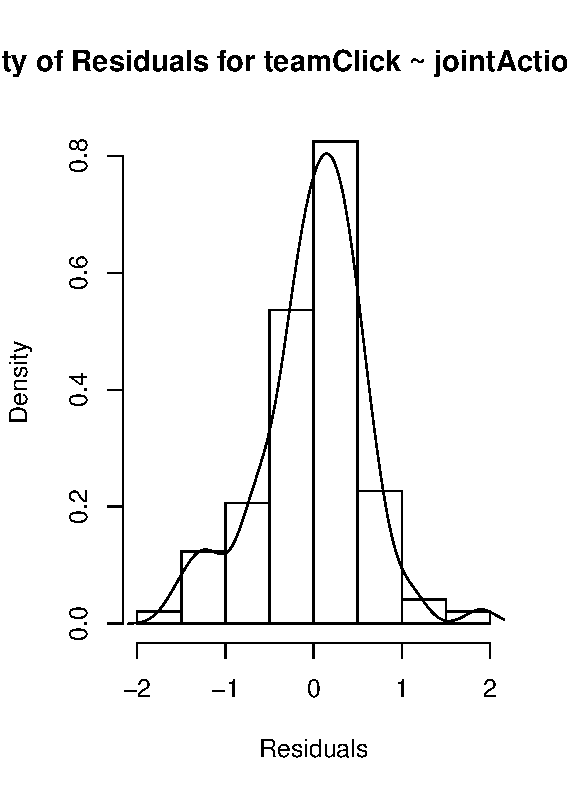
\includegraphics{../images/MLM1aHistResiduals.pdf}
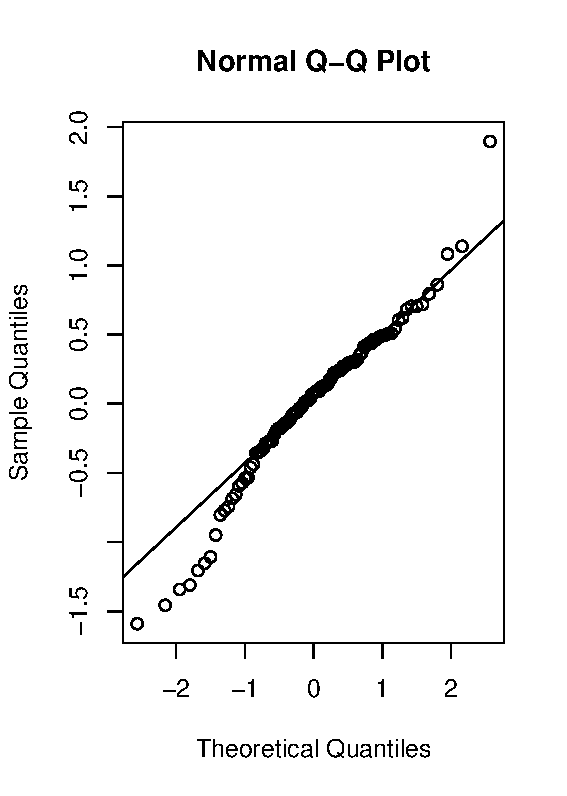
\includegraphics{../images/MLM1aQQNorm.pdf}
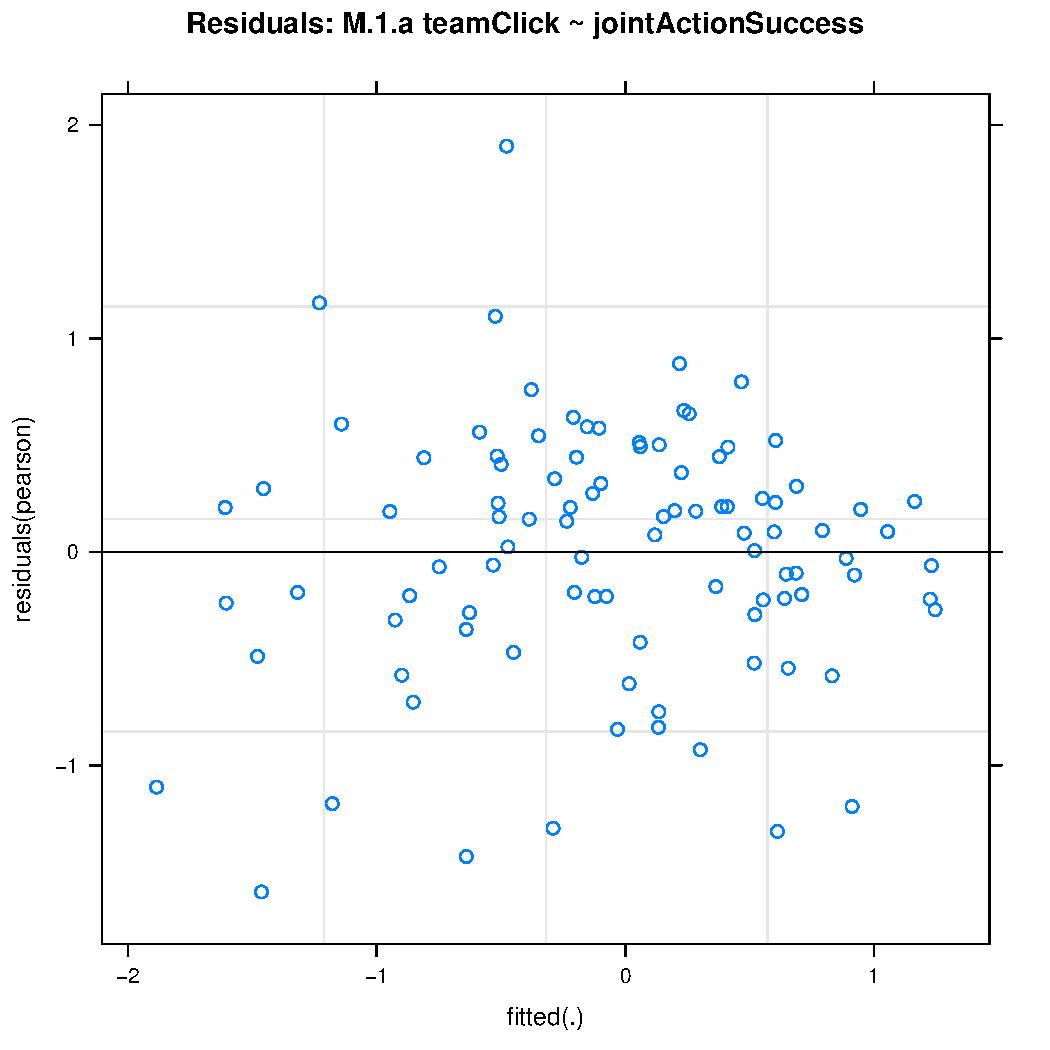
\includegraphics{../images/MLM1aScatter.pdf}
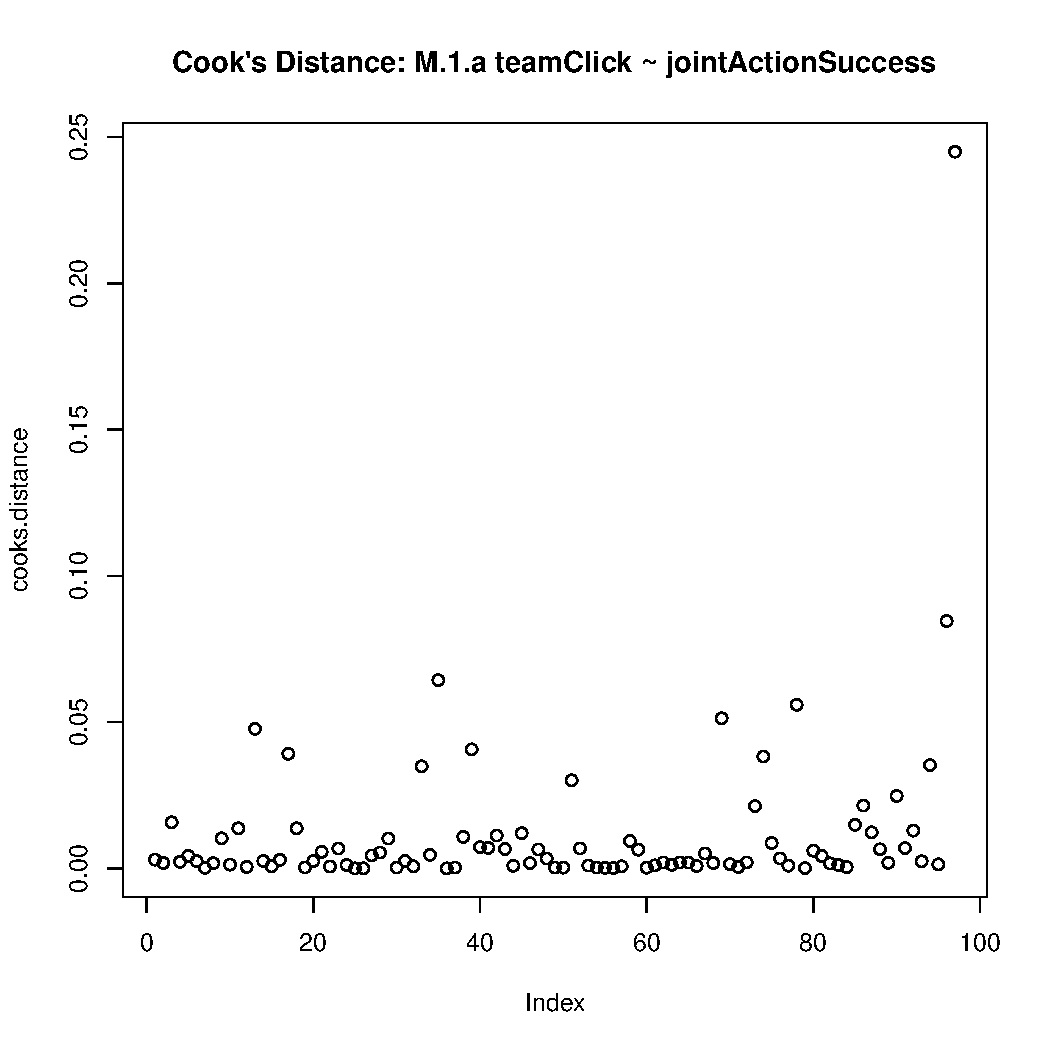
\includegraphics{../images/MLM1aCooksD.pdf}
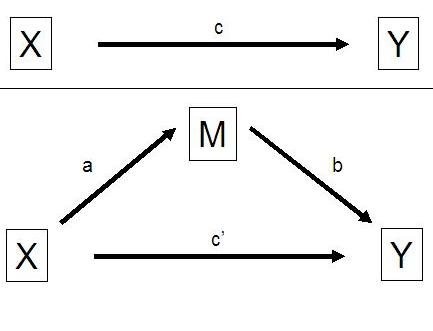
\includegraphics{../images/mediation_image.jpg}
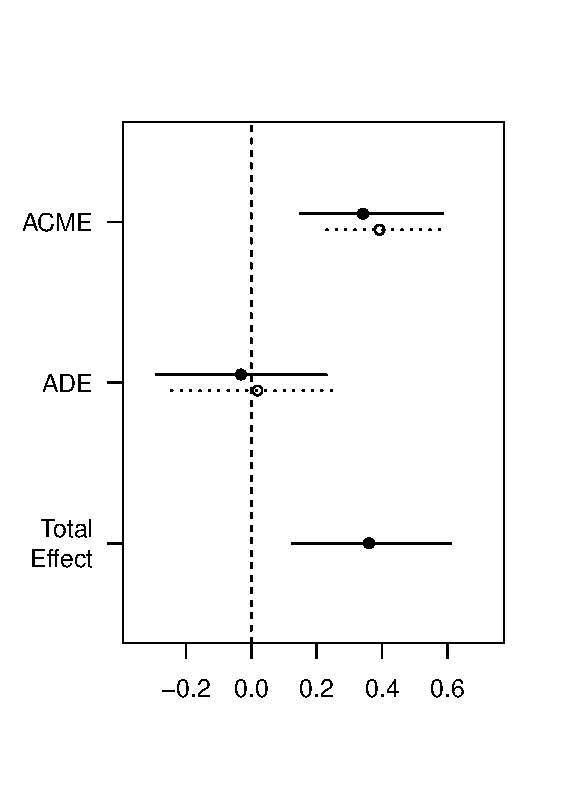
\includegraphics{../images/mediationPT_plot.pdf}

$$ ind = ab + \sigma_{a_{j}b_{j}} \quad (EQ:A11)$$

$$Var(ind) = b^{2} \sigma^{2}_{\hat{a}} + a^{2} \sigma^{2}_{\hat{b}} + \sigma^{2}_{\hat{a}}\sigma^{2}_{\hat{b}} + 2ab\sigma_{\hat{a},\hat{b}} + (\sigma_{\hat{a},\hat{b}})^2 + \sigma^{2}_{\hat{\sigma}_{a_{j},b_{j}}} \quad (EQ:A14) $$

average total effect

$$ tot = ab + \sigma_{a_{j}b_{j}} + c’ \quad (EQ:A15) $$ $$ Var(ind) = b^{2}\sigma^{2}_{\hat{a}} + a^{2}\sigma^{2}_{\hat{b}} + 2ab\sigma_{\hat{a},\hat{b}} + 2b\sigma_{\hat{a},\hat{c}’} + 2a\sigma_{\hat{b},\hat{c}’} + \sigma^{2}_{\hat{\sigma}_{a_{j},b_{j}}} + \sigma^{2}_{\hat{c}’} + \sigma^{2}_{\hat{a}}\sigma^{2}_{hat{b}} + (\sigma_{hat{a},hat{b}})^2 \quad (EQ:A18) $$


($Y \sim \beta_0 + \beta_1X + \epsilon$)

\begin{equation*}
  Y_i \sim \beta_0 + \beta_1X_i + \beta_2 M_i + \epsilon_i
\end{equation*}

blah blah blah\citep{Keller2014}

\printbibliography

\end{document}
